\documentclass[12pt]{article}
\usepackage{coursenote}
\begin{document}
\title{STAT 401 Chapter 8.1--8.3, 8.5}
\maketitle

\section{Polynomial regression models}

(Self reading.)

One predictor variable, second order:
\[
Y = \beta_0 + \beta_1 X + \beta_2 X^2 + \epsilon
.
\]
One predictor variable, third order:
\[
Y = \beta_0 + \beta_1 X + \beta_2 X^2 + \beta_3 X^3 + \epsilon
.
\]
Two predictor variables, second order:
\[
Y = \beta_0 + \beta_1 X_1 + \beta_2 X_2 + \beta_{11} X_1^2
    + \beta_{22} X_2^2 + \beta_{12} X_1X_2 + \epsilon
.
\]


\remark
1. In general, a $k$-th order polynomial can perfectly fit $k+1$ points.
For example, a straight line (first order) can be found to go exactly
through any two points on the $X-Y$ plane;
a quadratic curve (second order) can be found to go
exactly through any three points
(as long as the do not fall on a straight line).
For more points, a higher order polynomial may provide a good (or even
perfect) fit, but that does not mean the polynomial captures essential
relations between the predictor and response variables.
Other than the data points (and especially outside of data range),
the polynomial may have erratic curvature that is totally unrealistic.
Do not use a high order polynomial simply because it can fit.

2. Generally speaking,
forget about fourth and higher orders. Be wary of third order.

3. All the orders lower than the highest should be included
in the model.

4. Polynomials may demonstrate high collinearity, causing
difficulties in computing (near singular $\mat{X}'\mat{X}$).
Usual trick: use centered predictor variable.
That is,
use $X' = X - \overline{X}$ instead of $X$ itself.


\section{Modeling interactions}

Take the model
\[
E(Y) = \beta_0 + \beta_1 X_1 + \beta_2 X_2
\]
If $X_2$ is fixed, how does $E(Y)$ change with the value of $X_1$?
It's all in the slope of $X_1$:
\[
\Delta E(Y) = \beta_1 \cdot \Delta X_1
\]
regardless of the actual value of $X_2$ as long as it is fixed.

Now if the model is
\[
E(Y) = \beta_0 + \beta_1 X_1 + \beta_2 X_2 + \beta_{12}X_1X_2
\]
and $X_2$ is again fixed, then as $X_1$ changes,
\[
\Delta E(Y)
= \beta_1 \cdot \Delta X_1 + \beta_{12}X_2\cdot \Delta X_1
= (\beta_1 + \beta_{12}X_2) \cdot \Delta X_1
\]
The rate of the change in $E(Y)$ as $X_1$ changes
\emph{is} affected by the actual value of $X_2$.
In effect, $X_2$ affects the slope of $X_1$.

This phenomenon is \underline{interaction}
between $X_1$ and $X_2$. In the model above,
the interaction is accounted for by the crossproduct term
$\beta_{12}X_1X_2$.

This is a general strategy:
\underline{crossproduct terms represent interactions}.


\section{Qualitative predictors}

\example
The city tax assessor was interested in predicting residential home
sales prices in a mid-western city as a function of various
characteristics of the home and surrounding property.
Here we are interested in modeling sales price (\verb+Price+)
by the size (\verb+SquareFeet+),
with possible influence by the ``style'' (\verb+Style+) of the home.
There are 4 styles: A, B, C, and G.

We fitted the model separately for each style of home;
see plot.

\begin{figure}
\begin{center}
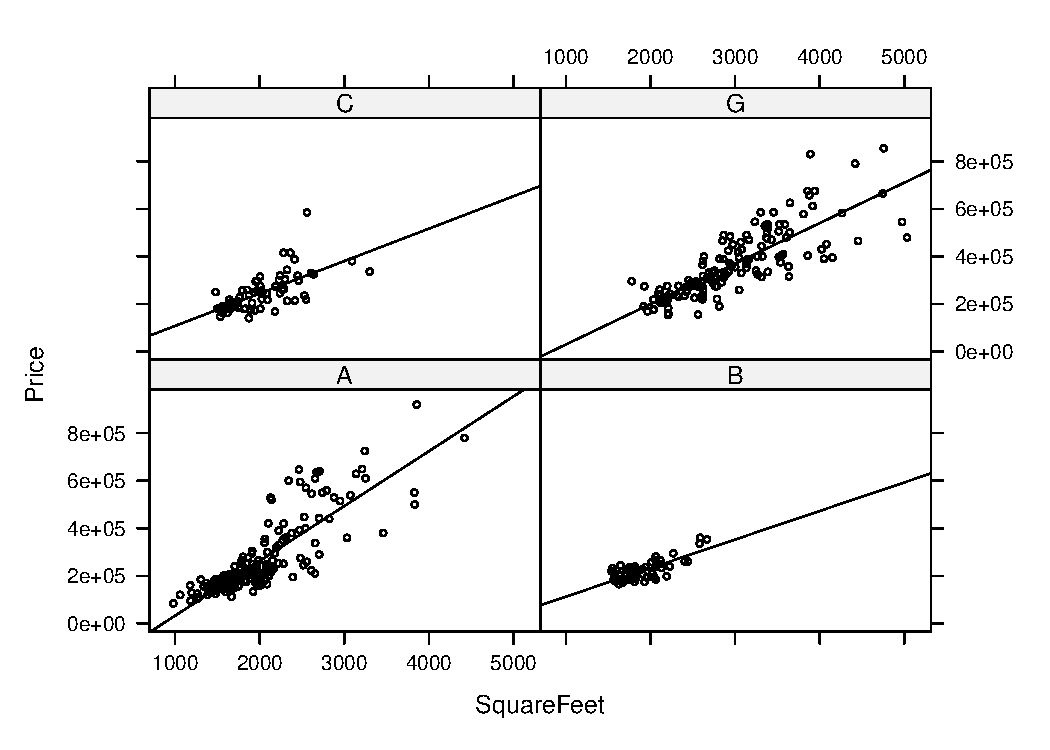
\includegraphics[width=.95\textwidth]{part11-sales.pdf}
\end{center}
\end{figure}

Instead of fitting a model for each style,
now we want to treat \verb+Style+ as a predictor, that is,
the model is\\
\verb&Price ~ SquareFeet + Style&.
\\
Problem is, \verb+Style+ is not numerical (or quantitative);
it is instead categorical (or qualitative).
How can we deal with its values
``A'', ``B'', ``C'', ``G''?

What about coding the values as 1, 2, 3, 4?

If we did that, the model would be
\[
E(\text{\tt Price})
= \beta_0
    + \beta_1 \cdot\text{\tt SquareFeet}
    + \beta_2 \cdot\text{\tt Style}
\]
Suppose the estimated function is
(whether or not the model is appropriate,
we can always soldier on and compute the estimates)
\[
E(\text{\tt Price})
= 1000
    + 210 \cdot\text{\tt SquareFeet}
    + 82 \cdot\text{\tt Style}
\]

We see at least two problems:
\begin{enumerate}
\item The model says the expected price increases
as the ``style'' goes from 1, to 2, to 3, and so on.
So the style has an order (in its relation to price).
Does this ordering make sense?
It might. But, what if our coding messed up the correct order?
For example, say everything else equal, the selling price goes up
from style ``A'' to ``C'' to ``G'' to ``B'',
but we have coded them 1, 3, 4, 2.
With this coding, (1) the contribution of the predictor
\verb+Style+ will be messed up; it may not show in the estimation;
I don't know how to interpret the coefficient;
(2) in the fitted model we wouldn't be
able to tell that the ``correct order'' should have been ``A'', ``C'', ``G'',
``B'' to begin with.

\item This model says that with \verb+SquareFeet+ fixed at some value,
style ``B'' will tend to outsell style ``A'' by 82,
style ``C'' will tend to outsell style ``B'' by 82, and so on.
The effect of \verb+Style+ changes in equal increments.
Does this have to be the case for this real estate problem?
No.
\end{enumerate}


A qualitative variable differs from a quantitative one in two
fundamental ways:
\begin{enumerate}
\item It does not have an ``order''.
\item It does not have a sense of ``distance''.
\end{enumerate}
It just has a bunch of possible values.
The values are just different---you can't say things like
``B'' is larger than ``A'' or the difference between ``G'' and ``B'' is
larger than that between ``A'' and ``B''.

(Some qualitative variables have ordered values, e.g. ``low'',
``middle'', ``high'', but they still don't have a clear meaning of
``distance''.)



\subsection{Binary coding for qualitative predictors}

We can let the role of the qualitative \verb+Style+ be played
by four \underline{indicator} variables in a concerted way:
\verb+StyleIsA+, \verb+StyleIsB+, \verb+StyleIsC+,
\verb+StyleIsG+.
Then the value of \verb+Style+ is replaced by the value of a length-4
vector:

\begin{tabular}{c|cccc}
\verb+Style+ & \verb+StyleIsA+ & \verb+StyleIsB+ & \verb+StyleIsC+
& \verb+StyleIsG+ \\ \hline
``A'' & 1 & 0 & 0 & 0\\
``B'' & 0 & 1 & 0 & 0\\
``C'' & 0 & 0 & 1 & 0\\
``G'' & 0 & 0 & 0 & 1\\ \hline
\end{tabular}

Now we can fit the model
\[
E(\text{\tt Price})
= \beta_0
    + \beta_1\cdot \text{\tt SquqreFeet}
    + \beta_A\cdot \text{\tt StyleIsA}
    + \beta_B\cdot \text{\tt StyleIsB}
    + \beta_C\cdot \text{\tt StyleIsC}
    + \beta_G\cdot \text{\tt StyleIsG}
\]
Each of the \verb+StyleIs*+ variables is binary,
taking values 0 and 1.
Combined they encode the information of \verb+Style+.
Their coefficients are not restricted by any ordering or equal
increments.

For any particular value of \verb+Style+ (say ``A''),
only one (\verb+StyleIsA+) indicator is 1 and the others are all 0.
The coefficient of the nonzero indicator will take effect in predicting
$Y$ at this value of \verb+Style+.
Pretty good.

Except for only one problem.

Think about the design matrix, in which each indicator occupies a
column.
The sum of these four columns is identical to the intercept column.
That is, these 5 columns are perfectly correlated:\\
\verb&StyleIsA + StyleIsB + StyleIsC + StyleIsG - X0 = 0&.\\
This is \emph{multicollinearity} and it will break the model.

Solution: we need only 3 indicators:

\begin{tabular}{c|cccc}
\verb+Style+ & \verb+StyleIsA+ & \verb+StyleIsB+ & \verb+StyleIsC+ \\ \hline
``A'' & 1 & 0 & 0 \\
``B'' & 0 & 1 & 0 \\
``C'' & 0 & 0 & 1 \\
``G'' & 0 & 0 & 0 \\ \hline
\end{tabular}

Style ``G'' is implied if the indicators for all the other styles are 0.


\subsection{Application examples}

1. Urban regions, rural regions.

2. War time, peace time.

3. 4 seasons (fiscal quarters).

4. 12 months.

5. Age groups.

6. A numerical variable cut into several ranges.
(Although it's a numerical variable, sometimes the actual number,
varying in a broad range, does not make good relation.
By cutting it into several segments, we discard the order
and other quantitative meanings but just treat the segments as
different. This seems to be losing information, but it could gain
in flexibility: better fitting could be achieved
than when certain quantitative relation is imposed yet
the model's form is not flexible enough
with this imposed relation.)


\section{Interactions between quantitative and qualitative predictors}

Quantitative and qualitative predictors can be present side by side.
They can also interact.

\example
$X_1$: size of insurance firm (number of employees; quantitative).\\
$X_2$: type of firm (stock/mutual; qualitative).\\
$Y$: speed of insurance innovation (quantitative).

\[
Y = \beta_0 + \beta_1 X_1 + \beta_2 X_2 + \beta_{12}X_1X_2 + \epsilon
\]
$X_2 = 1$ if stock firm and 0 if mutual firm.

\subsubsection{Interpretation}

Stock firm:
\[
Y = (\beta_0 + \beta_2) + (\beta_1 + \beta_{12}) X_1  + \epsilon
\]
Mutual firm:
\[
Y = \beta_0 + \beta_1 X_1  + \epsilon
\]

Suppose our focus is the relation between $Y$ and the quantitative
variable $X_1$,
but we also keep an eye on
how this relation is affected by the qualitative variable $X_2$.

The interaction term $\beta_{12} X_1 X_2$
changes the \emph{slope} of the $Y \sim X_1$ relation as $X_2$ takes
different values.

The term $\beta_2 X_2$
changes the \emph{intercept} of the $Y \sim X_1$ relation as $X_2$ takes
different values.

\example
Soap production lines, page 330--334.

\section{Computation}
\begin{verbatim}
> data <- read.table('RealEstateSales.txt', header = TRUE)
> data <- data[data$Style %in% c(1,2,3,7), ]
>     # Take the observations with styles numbered 1, 2, 3, 7
>     # because these several styles have more observations.
> data$Style <- LETTERS[data$Style]
>     # In the dataset 'Style' is a number.
>     # Change it to capital letters.
>     #  1, 2, 3, 7 => 'A', 'B', 'C', 'G'
> 
> print(names(data))
 [1] "ID"         "Price"      "SquareFeet" "NumBed"     "NumBath"   
 [6] "AC"         "GarageSize" "Pool"       "Year"       "Quality"   
[11] "Style"      "LotSize"    "Highway"   
> print(data$Style)
  [1] "A" "A" "A" "A" "G" "A" "G" "A" "A" "A" "G" "A" "G" "A" "A" "G" "G" "A"
 [19] "B" "A" "A" "C" "A" "A" "A" "G" "G" "A" "G" "A" "A" "A" "A" "C" "A" "A"

 (...omitted...)
> 
\end{verbatim}

Let's fit the model with predictors
\verb+SquareFeet+ and \verb+Style+.
Remember \verb+Style+ is now character values.
\begin{verbatim}
> print(lm(Price ~ SquareFeet + Style, data))

Call:
lm(formula = Price ~ SquareFeet + Style, data = data)

Coefficients:
(Intercept)   SquareFeet       StyleB       StyleC       StyleG  
  -126048.5        193.3     -20182.0     -18323.4     -83925.8  

Warning message:
In model.matrix.default(mt, mf, contrasts) :
  variable 'Style' converted to a factor
\end{verbatim}

\texttt{R} did the job but gave a warning, saying
it had converted \verb+Style+ to a ``factor''.

``Factor'' is the \texttt{R} data type for qualitative variables.
(Recall we have seen types of numericals, logicals, characters.)
We'd better do the conversion ourselves to be really in control of
what's going on:

\begin{verbatim}
> 
> data$Style <- factor(data$Style)
>     # Or 'as.factor' in this case.
\end{verbatim}

Now the factor-type variable \verb+Style+
has 4 ``levels'', with ``labels'' `A', `'B', `C', and `G'.
Since we didn't specify a particular order of the levels,
\texttt{R} will arrange them in the alphabetic order of the labels.

Now fit the model again:
\begin{verbatim}
> fit <- lm(Price ~ SquareFeet + Style, data)
> print(fit)

Call:
lm(formula = Price ~ SquareFeet + Style, data = data)

Coefficients:
(Intercept)   SquareFeet       StyleB       StyleC       StyleG  
  -126048.5        193.3     -20182.0     -18323.4     -83925.8  

> 
> print(summary(fit), digits = 2)

Call:
lm(formula = Price ~ SquareFeet + Style, data = data)

Residuals:
    Min      1Q  Median      3Q     Max 
-283825  -34741   -4269   29280  300404 

Coefficients:
            Estimate Std. Error t value Pr(>|t|)    
(Intercept) -1.3e+05    1.4e+04    -9.3   <2e-16 ***
SquareFeet   1.9e+02    6.5e+00    29.8   <2e-16 ***
StyleB      -2.0e+04    1.1e+04    -1.8     0.07 .  
StyleC      -1.8e+04    1.1e+04    -1.7     0.09 .  
StyleG      -8.4e+04    1.1e+04    -7.8    4e-14 ***
---
Signif. codes:  0 ‘***’ 0.001 ‘**’ 0.01 ‘*’ 0.05 ‘.’ 0.1 ‘ ’ 1 

Residual standard error: 75000 on 467 degrees of freedom
Multiple R-squared: 0.71,	Adjusted R-squared: 0.71 
F-statistic: 2.9e+02 on 4 and 467 DF,  p-value: <2e-16 
> 
\end{verbatim}

Note, \texttt{R} automatically replaced \verb+Style+ by 3 indicator
variables: \verb+StyleB+, \verb+StyleC+, \verb+StyleG+.
A little different from our encoding, but the idea is the same and the
result is equivalent.

We can guess \texttt{R}'s way of encoding a factor is
to skip the first level and create an indicator for each of the other
levels. When all the indicators are 0, it means the first level.

\end{document}

